% Created 2018-02-19 Mon 03:33
% Intended LaTeX compiler: pdflatex
\documentclass[a4paper,11pt]{article}
\usepackage[utf8]{inputenc}
\usepackage[T1]{fontenc}
\usepackage{graphicx}
\usepackage{grffile}
\usepackage{longtable}
\usepackage{wrapfig}
\usepackage{rotating}
\usepackage[normalem]{ulem}
\usepackage{amsmath}
\usepackage{textcomp}
\usepackage{amssymb}
\usepackage{capt-of}
\usepackage{hyperref}

% for code
\usepackage{minted}
\usepackage{mathtools}
\usepackage{siunitx}

% for footer
%\usepackage[symbol]{footmisc}
%\renewcommand{\thefootnote}{\fnsymbol{footnote}}

% for floating table
\usepackage[T1]{fontenc}
\usepackage[font=small,labelfont=bf,tableposition=top]{caption}
\DeclareCaptionLabelFormat{andtable}{#1~#2  \&  \tablename~\thetable}

% for table color
\usepackage{color}
\usepackage{booktabs}

\definecolor{red-1}{rgb}{1,0.6,0.6}
% \definecolor{green-1}{rgb}{0.7,1,0.6} / 0.1,1,0.5
\definecolor{green-1}{rgb}{0.5,1,0.5}
\definecolor{blue-1}{rgb}{0.4,0.7,1.0}
\definecolor{orange-1}{rgb}{1,0.7,0.4}

\author{Azzam Syawqi Aziz}
\date{\today}
\title{\emph{DISTRIBUTED VERSION CONTROL} DAN \emph{OPEN FORMAT}
  SEBAGAI SOLUSI PERMASALAHAN PADA TUGAS KOLABORATIF DI UNIVERSITAS.}
\hypersetup{
  pdfauthor={azzamsa},
  pdftitle={},
  pdfkeywords={},
  pdfsubject={},
  pdfcreator={Emacs 24.5.1 (Org mode 9.1.2)},
  pdflang={English}}
\begin{document}

\maketitle
%\tableofcontents


%\section{\emph{Distributed Version Control} dan \emph{Open Format}
%  sebagai solusi permasalahan pada tugas kolaboratif di Universitas.}
%\label{sec:orgae2306e}

Kerja kelompok sudah menjadi napas para mahasiswa di kampus. Terlebih
di fakultas yang memiliki mata kuliah dengan segudang proyek akhir.
Saya sendiri terbiasa mengerjakan porsi lebih banyak daripada teman
sekelompok. Keinginan untuk memahami materi lebih dalam dan kecintaan
pada \emph{computer science} membuat saya tidak terganggu, meskipun
saya harus mengerjakan tugas atau proyek akhir seorang diri.

{
\renewcommand*{\thefootnote}{\fnsymbol{footnote}}

Seiring berjalannya waktu, beberapa hal ganjal menghampiri. Kali ini
saya tak lagi tenang meskipun sudah terbiasa mengerjakan tugas akhir
seorang diri. Semester lalu, saya melihat Andi\footnote[1]{Nama
Fiktif} selalu marah dan mengeluh di kelas. Ia bercerita bahwa teman
sekelompoknya tidak pernah mau ikut andil dalam tugas kelompoknya.
Bahkan mereka membalas ajakan untuk kerja kelompok secara acuh. Maklum
saja karena memang tidak sedikit mahasiswa kampus yang lebih fokus
pada hal-hal di luar kampus.

}

\renewcommand*{\thefootnote}{\arabic{footnote}}
\setcounter{footnote}{0}

Berbeda dengan Andi yang berani menghapus nama teman yang tak aktif
bekerja, Budi* lebih memilih untuk diam. Saya selalu diliputi rasa iba
tatkala bertemu dengannya di kelas. Kali ini teman-temannya tidak
membantu bukan karena acuh, melainkan karena mereka tidak paham
bagaimana cara mengerjakan tugas tersebut.

Begitu pun Ani* yang secara lugas menjawab "sudah biasa", tatkala
ditanya mengapa ia bekerja sendiri. Pada awalnya saya pikir hal-hal
ini mungkin hanya terjadi pada beberapa teman saya saja. Tetapi
munculnya banyak \emph{post} di sosial media yang mengeluhkan bahwa
teman mereka tidak pernah ikut bekerja atau hanya muncul ketika
ditanya nomor induk mahasiswa, membuat saya merasa permasalahan ini
harus memiliki solusi.


% \subsection{Jumlah yang tidak sedikit}
\section{Jumlah yang tidak sedikit}
\label{sec:statistic}

Hasil mengejutkan terlihat pada data yang dihimpun dari $\pm 100$
responden dari total $\pm 800$ populasi menghasilkan statistik berikut.

\begin{center}
  \textbf{\small Berapa kali anda mengerjakan tugas kelompok seorang diri ?}
\end{center}

% \begin{figure}[tp]
%   \begin{figure}[!htb] works
\begin{figure}[!ht]
  \centering
  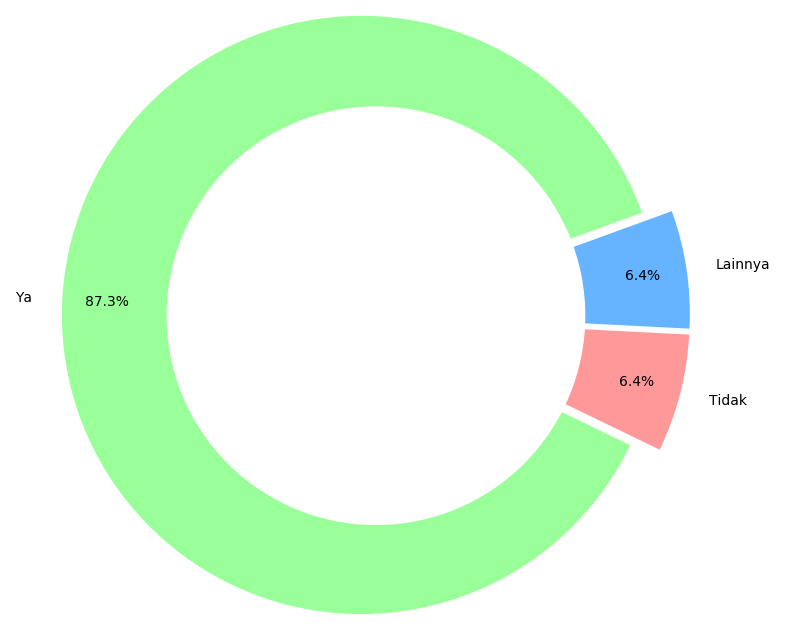
\includegraphics[width=.4\linewidth]{img/kerja-sendiri-1.png}
  \qquad
  \begin{tabular}[b]{cc}\hline
    Respons & Persentase \\ \hline
    \color{green-1}{Ya} & $\SI{87.3}{\percent}$ \\
    \color{red-1}{Tidak} & $\SI{6.4}{\percent}$  \\
    \color{blue-1}{Lainnya} & $\SI{4.0}{\percent}$ \\ \hline
  \end{tabular}
  \captionlistentry[table]{berapa kali bekerja sendiri}
  \captionsetup{labelformat=andtable}
    \caption{berapa kali bekerja sendiri}
\end{figure}

Sebanyak $\SI{87}{\percent}$ dari responden pernah bekerja sendiri
dalam proyek akhir mata kuliah tertentu yang seharusnya dikerjakan
secara berkelompok. Artinya \textbf{jika diambil 10 orang secara acak
dari 800 orang, maka setiap 10 orang ada 8 orang yang mengerjakan
tugas kelompoknya seorang diri}. Diantaranya rata-rata pernah bekerja
sendirian mulai 1 hingga lebih dari 5 kali.

Dengan kata lain, jika 800 dari populasi dikelompokkan dengan maksimal
5 orang, maka terdapat total 160 kelompok, \textbf{sehingga terdapat
$\pm 139$ kelompok dari 160, dimana di dalamnya ada seorang anak yang
mengerjakan tanpa bantuan yang lain}. Pada data ini terdapat
kemungkinan seseorang bekerja pada tim A sendirian, namum tidak aktif
di tim B.

Ada hal tak biasa yang saya temukan pada bagian ``Apakah ada yang
ingin anda sampaikan ?''. Tidak sedikit diantara mereka yang meminta
tolong dan berharap ada solusi untuk masalah ini. Tidak jarang
pula ada yang mendukung dan memberikan semangat dengan harapan riset
kecil ini dapat membuahkan hasil.

\begin{center}
  \textbf{\small Apakah dosen anda mengetahui bahwa anda bekerja sendiri ?}
\end{center}

\begin{figure}[!ht]
  \centering
  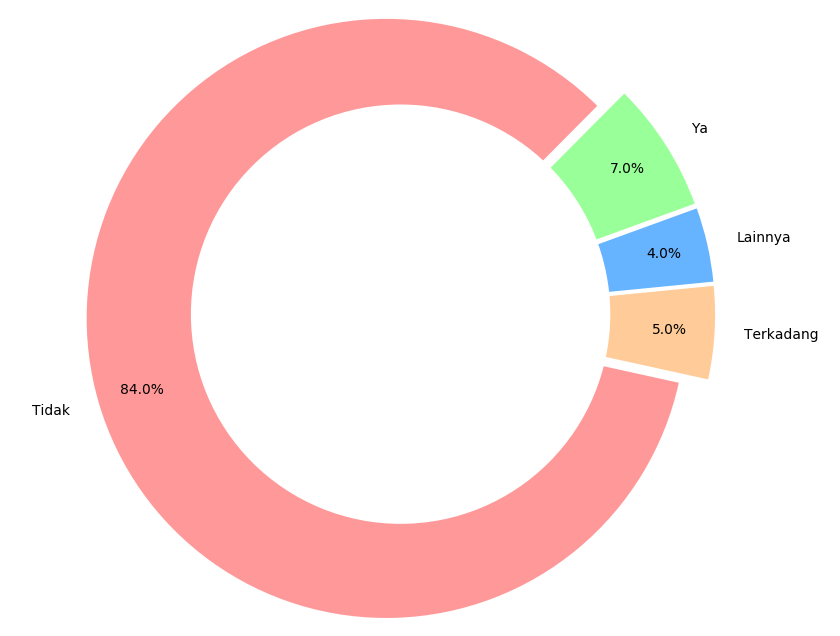
\includegraphics[width=.4\linewidth]{img/dosen-tau-2.png}
  \qquad
  \begin{tabular}[b]{cc}\hline
    Respons & Persentase \\ \hline
    \color{red-1}{Tidak} & $\SI{84.0}{\percent}$ \\
    \color{green-1}{Ya} & $\SI{7.0}{\percent}$  \\
    \color{orange-1}{Terkadang} & $\SI{5.0}{\percent}$ \\
    \color{blue-1}{Lainnya} & $\SI{4.0}{\percent}$ \\ \hline
  \end{tabular}
  \captionlistentry[table]{apakah dosen tau}
  \captionsetup{labelformat=andtable}
  \caption{apakah dosen tau}
\end{figure}


Tentu para mahasiswa tidak mungkin menyampaikan hal ini kepada dosen,
dengan berbagai macam alasan. Harapan kedepannya, data yang dihasilkan
dari alur kerja essay ini dapat membantu dosen memberikan hak kepada
mereka yang berhak, serta membangun suasana yang sehat dan sportif di
lingkungan Universitas.

\section{\emph{Version control}\cite{wiki-git} dan \emph{Open format}\cite{wiki-of}.}
\label{sec:org3d84a5f}

Kedua alat ini akan memberikan banyak jawaban terhadap permasalahan
kerja kelompok yang kerap kali terjadi, ditinjau dari segi popularitas
\emph{version control} yang kerap kali digunakan adalah git, dan
\LaTeX atau Markdown untuk \emph{open format}.

Penggunaan \emph{open format} membuat git lebih mudah untuk melacak
perubahan, melihat statistik kontribusi, sejarah perubahan, maupun
waktu perubahan berkas. Singkatnya git membantu kita dalam menjawab
\textbf{oleh siapa dan kapan}.

Awalnya mahasiswa dituntut untuk mempelajari metodologi dari kedua
alat tersebut, mempelajari alat baru tentu membutuhkan investasi
waktu, senada dengan apa yang disampaikan Miyamoto
Musashi\cite{wiki-musashi} bahwa semua hal pada awalnya memang
sulit. Namun, penguasaan teknis \emph{version control} sudah
seharusnya dikuasai oleh mahasiswa ilmu komputer\cite{might}.

Tanpa kita sadari, kini git tak hanya terbatas penggunaannya pada
civitas akademika ilmu komputer dan para pengembang perangkat lunak
untuk melakukan kolaborasi, begitu pun \LaTeX yang sudah dikuasai oleh
banyak elemen masyarakat untuk menulis karya ilmiah dan berbagai hal
lain, penggunaan bahasa markah seperti Markdown sudah marak digunakan
untuk berkolaborasi di wiki, berkomentar di sosial media, maupun untuk
menulis artikel \emph{blog}.


\section{Penggunaan Alat}
\label{sec:org72910a8}

Git memiliki banyak fitur, tetapi hanya sebagian fitur yang akan
digunakan pada penyelesaian permasalahan ini.

Untuk melihat banyaknya statistik kontribusi seseorang pada sebuah
berkas, kita dapat melakukannya dengan cara:

\begin{minted}[breaklines,linenos,frame=lines]{bash}
git shortlog -sn --no-merges
\end{minted}

\begin{figure}[tp]
  \centering
  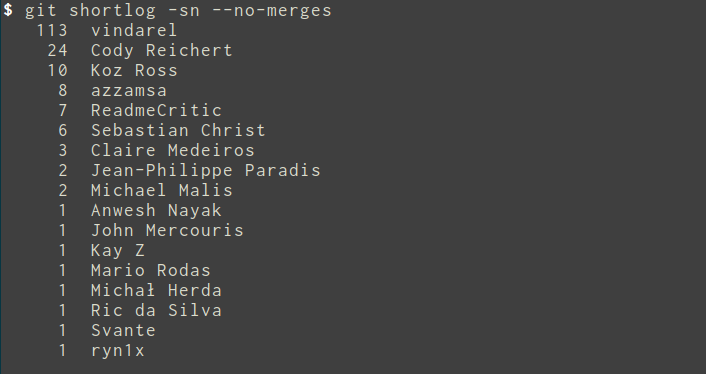
\includegraphics[width=.9\linewidth]{img/fig-1.png}
  \caption{git shortlog tanpa merge}
\end{figure}

\noindent
Melihat log perubahan berkas berdasarkan waktu. (Figure \ref{fig:git-log})

\begin{minted}[breaklines,linenos,frame=lines]{bash}
git log --pretty=custom
\end{minted}

\begin{figure}[tp]
  \centering
  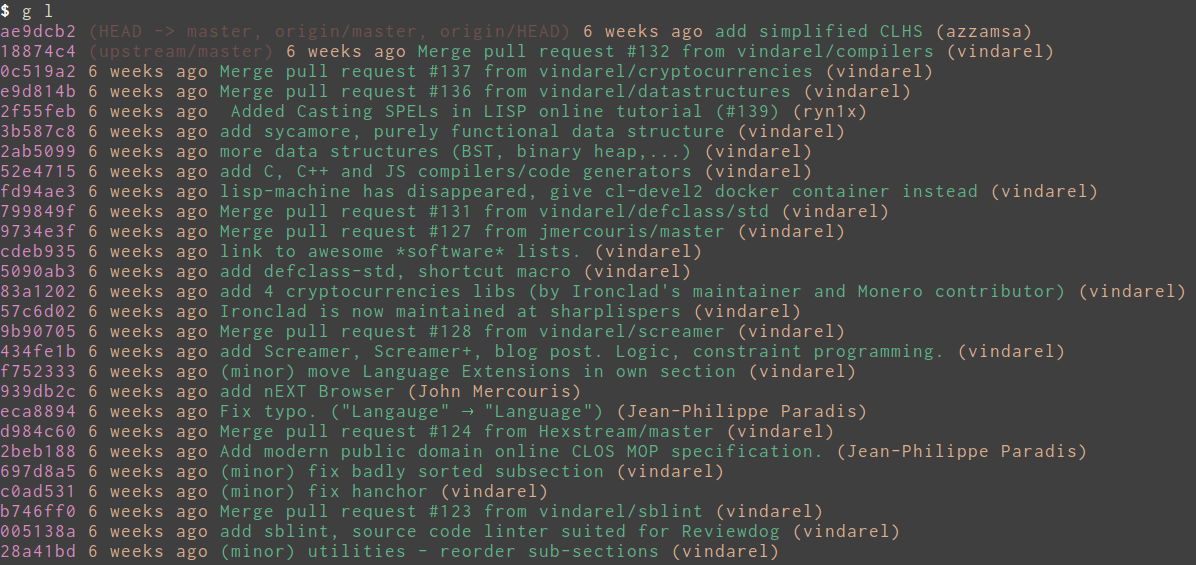
\includegraphics[width=.9\linewidth]{img/fig-2.png}
  \caption{git log}
  \label{fig:git-log}
\end{figure}

\noindent
Melihat siapa penulis pada baris tertentu. (Figure \ref{fig:git-blame})

\begin{minted}[breaklines,linenos,frame=lines]{bash}
git blame foo.txt
\end{minted}

\begin{figure}[tp]
  \centering
  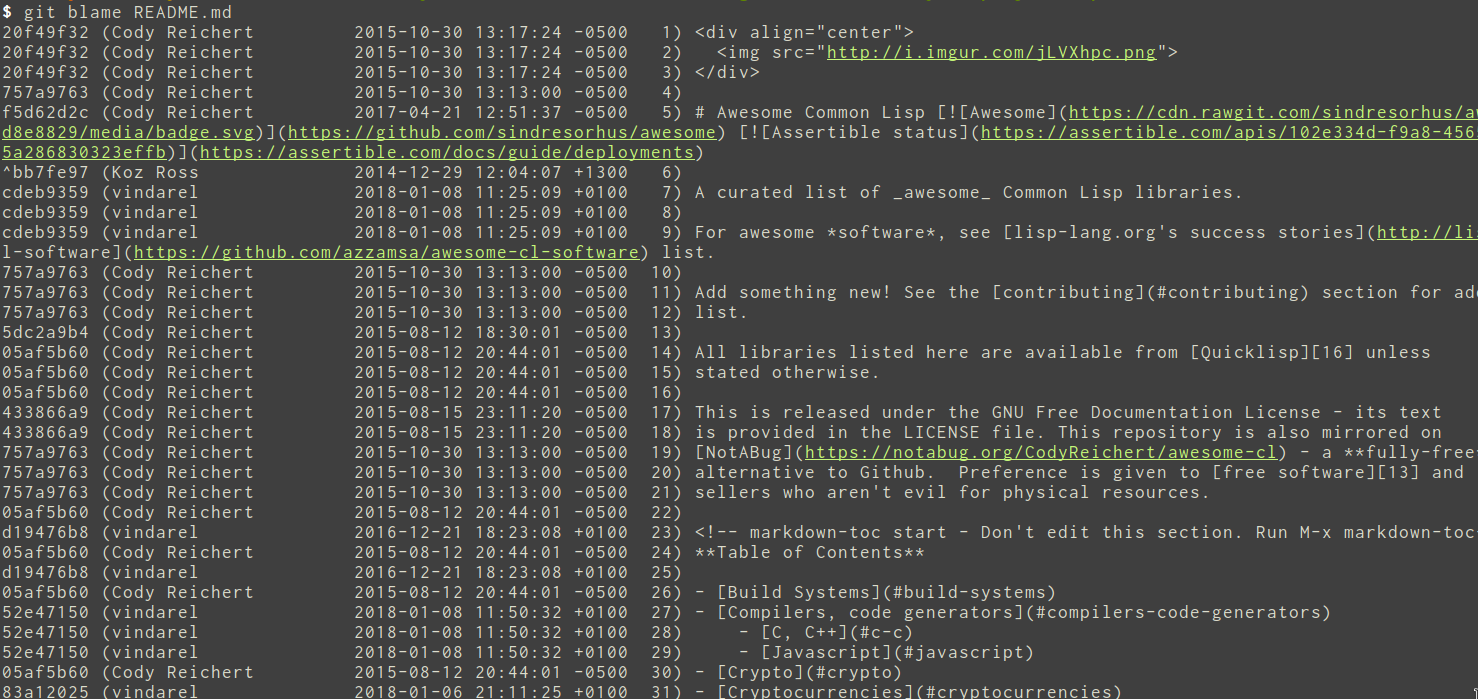
\includegraphics[width=.9\linewidth]{img/fig-4.png}
  \caption{git blame}
  \label{fig:git-blame}
\end{figure}

\noindent
Git sangat popular sehingga banyak fitur dari git di dukung oleh alat-alat lain,
seperti menggunakan magit di GNU Emacs. (Figure \ref{fig:magit})

\begin{minted}[breaklines,linenos,frame=lines]{bash}
M-x magit-blame
\end{minted}

\begin{figure}[tp]
  \centering
  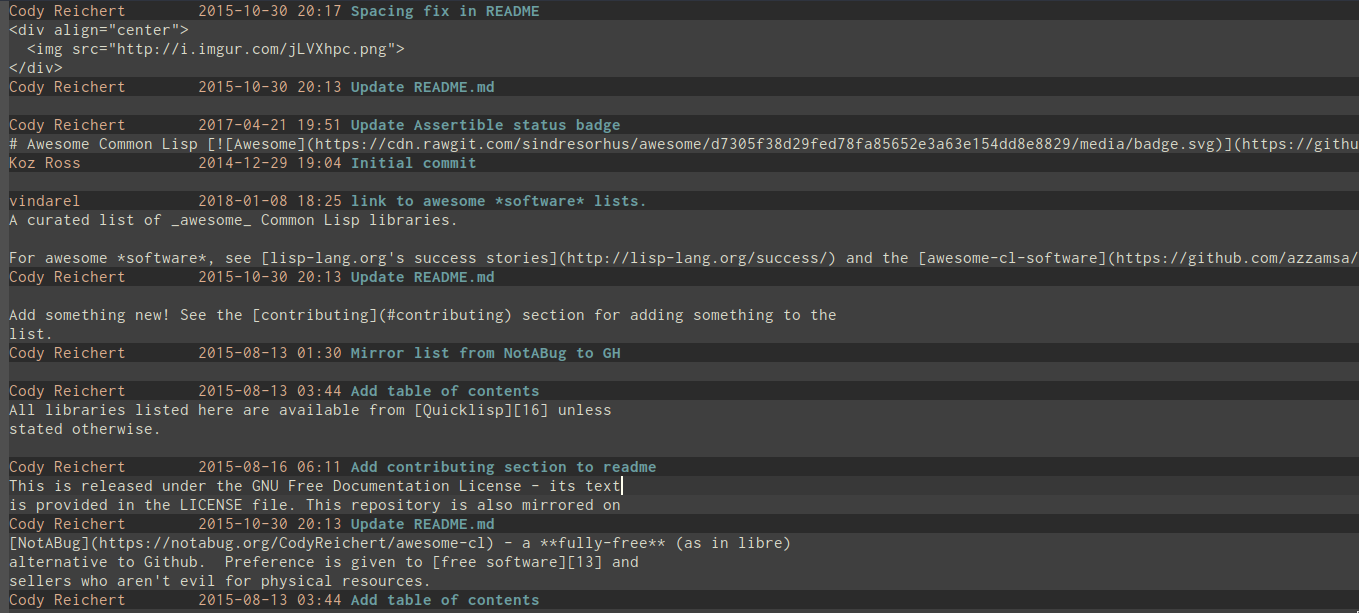
\includegraphics[width=.9\linewidth]{img/fig-5.png}
  \caption{magit-blame}
  \label{fig:magit}
\end{figure}

Banyak hal yang bisa kita lihat dari data yang dimiliki git hanya
menggunakan git ataupun dengan kombinasi alat-alat di lingkungan
GNU/Linux, seperti untuk melihat jumlah penghapusan dan penambahan baris. (Figure \ref{fig:git-awk})

\begin{minted}[breaklines,linenos,frame=lines]{bash}
git log --shortstat --author="azzamsa"  | grep -E "fil(e|es) changed" | awk -f lines.awk
\end{minted}

\begin{minted}[breaklines,linenos,frame=lines]{awk}
% lines.awk
{
  files+=$1;
  inserted+=$4;
  deleted+=$6;
}
END {
  print "files changed : ", files
  print "lines inserted: ", inserted
  print "lines deleted : ", deleted
}
\end{minted}


\begin{figure}[tb]
  \centering
  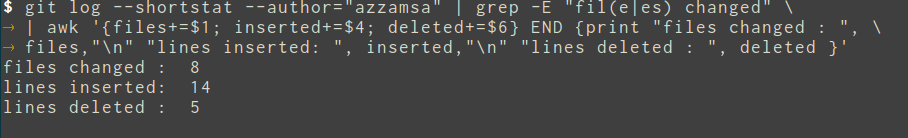
\includegraphics[width=.9\linewidth]{img/fig-3.png}
  \caption{git dengan alat Unix}
  \label{fig:git-awk}
\end{figure}

Alat-alat di atas akan lebih \emph{powerfull} jika dikombinasikan
dengan alat lainnya, seperti
\href{https://github.com/tomgi/git\_stats}{git\_stats},
\href{https://github.com/hoxu/gitstats}{gitstats}, atau
\href{https://github.com/ejwa/gitinspector}{gitinspector}. Selain
memiliki fitur-fitur yang baik untuk membuat laporan statistik, semua
alat yang disebutkan di atas berlisensi bebas\cite{wiki-fs}.

Kali ini saya hanya akan memperagakan penggunaan gitinspector, dengan
berkas dari \emph{repository}
\href{https://github.com/CodyReichert/awesome-cl}{awesome-cl}.

Menggunakan gitinspector dengan parameter \texttt{-r} untuk
menampilkan seberapa besar tanggung jawab (\emph{resposible}) seorang
pengarang terhadap suatu berkas. (Figure \ref{fig:gi-r})

\begin{minted}{bash}
gitinspector --file-types=md --format=html -r > hasil.html
\end{minted}

\begin{figure}[tp]
  \centering
  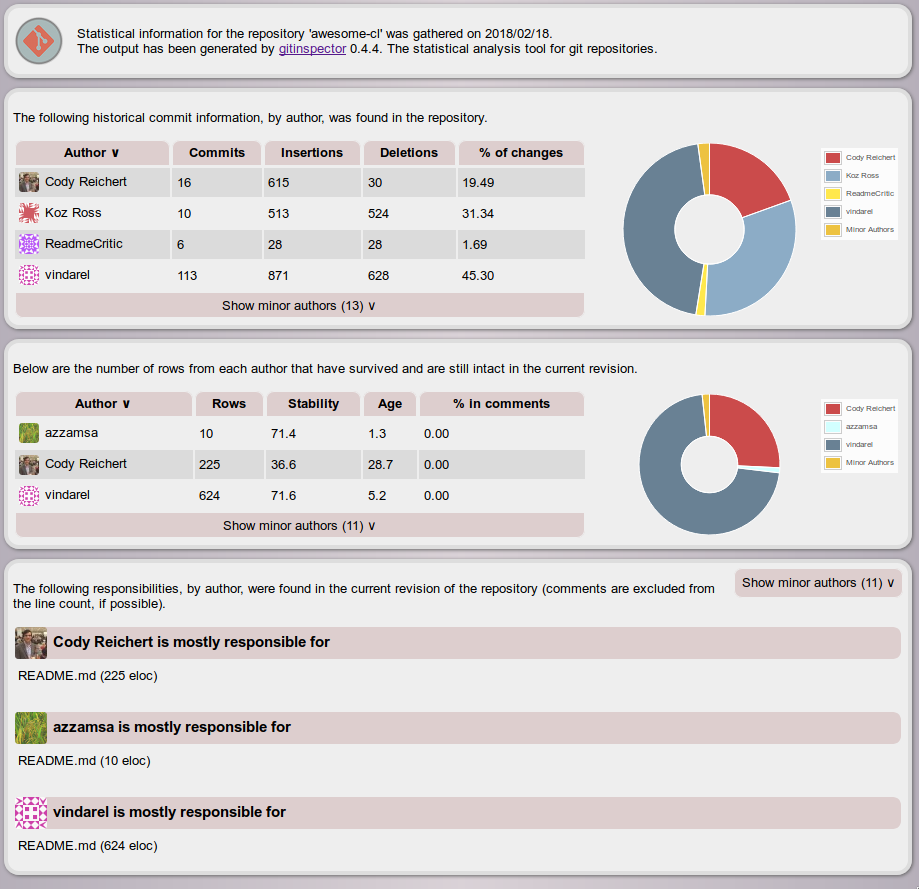
\includegraphics[width=.8\linewidth]{img/gi-1.png}
  \caption{gitinspector resposible}
  \label{fig:gi-r}
\end{figure}

\noindent
Menampilkan pekerjaan menurut waktu. (Figure \ref{fig:gi-t})

\begin{minted}[breaklines]{bash}
gitinspector --file-types=md --format=html -r -T --since=2017-01-01 > hasil.html
\end{minted}

\begin{figure}[tp]
  \centering
  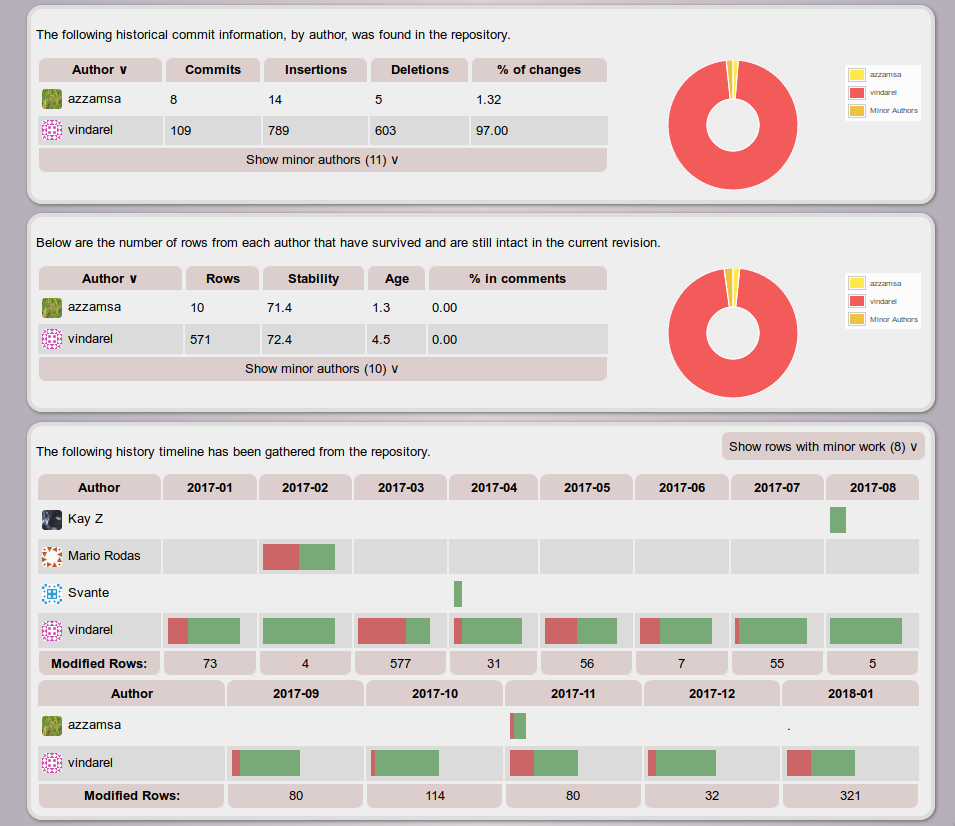
\includegraphics[width=.8\linewidth]{img/gi-2.png}
  \caption{gitinspector dengan \emph{history}}
  \label{fig:gi-t}
\end{figure}

Berkas yang dihasilkan gitinspector berbentuk HTML, JSON, atau pun
plain text. HTML yang dihasilkan mengandung javascript, sehingga
kontennya dinamis. Kita dapat melakukan perubahan urutan dengan
melakukan klik pada \emph{header} setiap kolom. Masih banyak fitur
lain yang dimiliki gitinspector\cite{gi-docs}, tetapi tentunya tidak
cukup untuk saya tampilkan semua di sini.

\section{Alat yang lebih mudah}
\label{sec:alat-mudah}

\LaTeX memiliki beragam pengolah berkas berlisensi bebas yang mudah
digunakan, seperti \href{http://www.xm1math.net/texmaker/}{texmaker}
dan \href{https://www.texstudio.org/}{texsutdio}. Begitu pun dengan
git yang memiliki banyak dukungan pihak ketiga yang memudahkan
penggunaannya, beberapa diantaranya disebutkan langsung oleh
pengembang git di daftar git GUI clients\cite{git-clients}.

Markdown dapat digunakan sebagai alternatif, jika \LaTeX dirasa
menelan waktu lebih lama untuk diadopsi, proses ekspor Markdown
kedalam bentuk PDF dapat dilakukan dengan pandoc.

\section{Timbulnya banyak manfaat lain}
\label{manfaat-lain}

Jika penggunaan \emph{open/libre format} serta \emph{version control}
sudah menjadi budaya di sebuah lingkungan Universitas, hal ini dapat
memberikan banyak manfaat lain, seperti:

\begin{itemize}
\item Penulisan tugas-tugas besar seperti skripsi maupun proyek akhir
  sudah tidak lagi menggunakan \emph{versioning manual} seperti ``tugas
  1 fix, tugas 1 fix sekali, tugas 1 final''.
\item Dosen dapat dengan mudah memastikan orisinalitas pekerjaan
  mahasiswa dengan melihat \emph{log}, \emph{commit
    sign}\cite{gitbook2}, dan bertanya melalui \emph{history}
  perubahan-perubahan yang dilakukan. Sehingga orisinalitasnya dapat
  dengan mudah dilacak dengan membaca pola pikir mahasiswa dalam
  melakukan perubahan-perubahan tersebut.
\item Penggunaan \emph{Open/libre format} dapat mengangkat wibawa dan
  nama Universitas.  Karena sudah seharusnya Universitas mengajarkan
  kepada mahasiswa tentang berkarya dan berkolaborasi. Dengan
  mengajarkan mahasiswa tentang perangkat lunak bebas, Universitas dapat
  mencetak lulusan yang siap terjun dalam masyarakat digital yang
  bebas. Ini akan membantu masyarakat secara keseluruhan untuk keluar
  dari dominasi oleh perusahaan-perusahaan besar\cite{stallman03}.
  Stallman juga menambahkan bahwa Universitas seharusnya mendukung
  penggunaan perangkat lunak bebas. Karena alat-alat tersebut
  berkontribusi untuk ilmu pengetahuan, layaknya universitas mendorong
  para mahasiswa dan ilmuwan untuk mempublikasikan karya mereka.
\item Universitas terbebas dari \emph{vendor lock-in}, dan memberikan
  kebebasan kepada mahasiswa untuk menggunakan alat apa pun, tanpa
  harus menggunakan alat \emph{proprietary}\cite{wiki-nonfs} tertentu. Mahasiswa tidak
  lagi diberatkan dengan proses pengumpulan dengan ekstensi tertentu dan
  versi tertentu.
\item Mahasiswa ilmu komputer yang memiliki lingkungan kampus dengan penggunaan
  alat-alat bebas, membuat mahasiswa termotivasi untuk menjelajahi alat-alat
  bebas lainnya, membaca kode sumbernya, dan mempelajari integrasi antara suatu
  alat dengan alat yang lain.
\end{itemize}

Beberapa hal di atas tentunya hanyalah sebagian dari banyak manfaat
lainnya, jika suatu Universitas memiliki lingkungan belajar yang baik
dan kolaborasi antar mahasiswa yang tinggi, tentu para mahasiswa akan
termotivasi untuk selalu mempelajari bagaimana sesuatu
bekerja. Perangkat lunak bebas mewadahi mereka untuk mempelajari cara
kerja alat-alat tersebut. Sehingga motivasi mereka untuk belajar,
berkarya dan berkontribusi kepada masyarakat semakin tinggi.

\section{Harapan}
\label{sec:org51ee297}

Dengan menggunakan alat-alat di atas, saya berharap teman-teman yang
sebelumnya banyak keteteran dalam mengerjakan tugas karena tidak
mendapat bantuan sedikit pun dari kelompoknya, teman-teman yang
seringkali meminta izin untuk telat mengumpulkan karena mengerjakan
sendiri, teman-teman yang selalu sayu wajahnya karena temannya aktif
berteriak lantang di luar kelas tetapi acuh dengan tanggung jawabnya
di kelas, bisa mendapatkan hak nya. Karena kita harus memberikan hak
kepada orang orang yang berhak, ucap Salman Al-farisi\cite{wiki-salman}.

Penilaian para dosen berbeda-beda. Jika alur kerja menggunakan alat di
atas dijadikan standar, maka dosen dengan proses penilaian spesifik
dan berdasar pada jumlah kontribusi, bisa menjadikannya sebagai acuan.
Sebaliknya dosen yang memberikan nilai yang sama pada setiap anggota,
terlepas ikut andil atau tidaknya seseorang pada suatu kelompok, dapat
mengabaikan data yang ada, meskipun hal ini tentunya tidak kita
harapkan. Kita tidak ingin lagi ada teman-teman yang merasa tidak
mendapat keadilan.

Saya berharap data yang dihasilkan tidak untuk menjerumuskan
teman-teman yang jarang berkontribusi dan menjadikan raja bagi para
mahasiswa yang mencintai bidang keilmuannya, tetapi bisa bersama
membangun, belajar, berbagi, berkarya, saling menolong, saling
mengajak dan mengajari.

Saya yakin dengan adanya hal ini, para mahasiswa yang belum memiliki
\emph{inner motivation} akan terpaksa pada awalnya untuk mengikuti
standar yang ada, dan bersyukur di kemudian hari atas ilmu yang
didapat.

Semoga alur kerja ini bisa digunakan dan bermanfaat untuk banyak
kalangan, dan semakin meningkat seiring berjalannya waktu.

\section{\emph{Credit}}
\label{sec:credit}
\begin{itemize}
\item Donald Knuth dan kotributor \href{https://www.tug.org/svn/texlive/trunk/}{\TeX}.
\item Leslie Lamport dan kontributor \href{https://www.latex-project.org/}{\LaTeX}.
\item Linus Torvalds, Junio Hamano dan kontributor \href{https://git-scm.com/}{git}.
\item John Gruber dan Aaron Swartz sebagai pengembang \href{https://daringfireball.net/projects/markdown}{Markdown}.
\item John MacFarlane dan kontributor sebagai pengembang \href{https://pandoc.org/}{pandoc}.
\item Adam Waldenberg dan kontributor sebagai pengembang \href{https://github.com/ejwa/gitinspector}{gitinspector}.
\item Marius Vollmer, Jonas Bernoulli dan kontributor sebagai pengembang \href{https://magit.vc/}{Magit}.
\end{itemize}


% \section{Referensi}
% \label{sec:org8bdc6d0}

\begin{thebibliography}{99}
\bibitem{wiki-git}
  Distributed version control.
  (n.d.).
  Didapat Februari 20, 2018, dari https://en.wikipedia.org/wiki/Distributed\_version\_control
\bibitem{wiki-of}
  List of open formats.
  (n.d.).
  Didapat Februari 20, 2018, dari https://en.wikipedia.org/wiki/List\_of\_open\_formats
\bibitem{wiki-musashi}
  Miyamoto Musashi.
  (n.d).
  Didapat Februari 20, 2018 dari https://en.wikipedia.org/wiki/Miyamoto\_Musashi
\bibitem{might}
  Might, M.
  (n.d.).
  What every computer science major should know.
  Didapat Februari 20, 2018 dari http://matt.might.net/articles/what-cs-majors-should-know/
\bibitem{wiki-fs}
  Free software license.
  (n.d.).
  Didapat Februari 20, 2018, dari https://en.wikipedia.org/wiki/Free\_software\_license
\bibitem{gi-docs}
  Gitinspector Docs.
  (n.d.).
  Didapat Februari 20, 2018. dari https://github.com/ejwa/gitinspector/blob/master/docs/gitinspector.pdf
\bibitem{git-clients}
  git GUI clients.
  (n.d.).
  Didapat Februari 20, 2018. dari https://git-scm.com/download/gui/linux
\bibitem{gitbook2}
  Straub, B dan Chacon S.
  (2014).
  \emph{Pro Git} (pp. 272-276).
  New York City, NY USA: Apress.
\bibitem{stallman03}
  Stallman, R.
  (2003).
  \emph{Free Software, Free Society: Selected Essays of Richard M. Stallman} (pp. 57-58).
  Boston, MA USA: GNU Press.
\bibitem{wiki-nonfs}
  Proprietary software.
  (n.d.).
  Didapat Februari 20, 2018 dari https://en.wikipedia.org/wiki/Proprietary\_software
\bibitem{wiki-salman}
  Salman Al-farisi.
  (n.d.).
  Didapat Februari 20, 2018. dari https://en.wikipedia.org/wiki/Salman\_the\_Persian
\end{thebibliography}

\end{document}
